\setcounter{Exercise}{0}
\section*{Algorithmes des parcours d'arbres binaire}
On peut implémenter un arbre binaire en Python en utilisant la POO. On crée une classe d'arbre binaire comme ci-dessous :
\begin{lstlisting}{style=pythonstyle, language=Python}
class ArbreBinaire:
    def __init__(self, valeur, gauche = None, droit = None):
        self.valeur = valeur  # Étiquette
        self.gauche = gauche  # Sous-arbre gauche
        self.droit = droit    # Sous-arbre droit
\end{lstlisting}
Pour la suite des exercices, nous considérerons toujours cette implémentation de la classe arbre.

\begin{Exercise}[title={Dessinons}]

\Question Dessiner l'arbre correspondant au code ci-dessous.\\
\emptybox{5cm}
\begin{lstlisting}{style=pythonstyle, language=Python}
B = ArbreBinaire("B")
C = ArbreBinaire("C")
D = ArbreBinaire("D", B, None)
K = ArbreBinaire("K", None, C)
Z = ArbreBinaire("Z")
E = ArbreBinaire("E", K, Z)
I = ArbreBinaire("I", D, E)
\end{lstlisting}

\Question Que vaut I.droit.gauche.valeur ?\\
\emptybox{1cm}
\Question Donner la ligne de code pour afficher la valeur de B avec I comme seule variable.\\
\emptybox{1cm}

\Question Compléter le code ci-dessous permettant de créer l'arbre avec une seule variable  ?\\
\begin{lstlisting}{style=pythonstyle, language=Python}
I = ArbreBinaire("I",
        ArbreBinaire("D",
            ArbreBinaire("B"),
            None),
        ArbreBinaire("E",
            ......................
                ....................
                ....................
            .....................)
            )    
\end{lstlisting}
\end{Exercise}

\vfill

\begin{Exercise}[title={Parcours infixe et suffixe}]

    \Question Compléter le code du parcours infixe ci-dessous.
    \begin{lstlisting}[style=pythonstyle, language=Python]
def parcours_infixe(self):
    if self.gauche is not None:
        self.gauche.parcours_infixe()
    print(self.valeur,end='-')
    if .....................................:
        ..................................................
    \end{lstlisting}
    \Question Que faut-il changer pour transformer le code ci-dessus en parcours suffixe ?\\
    \emptybox{4cm}
\end{Exercise}

%\vfill

\begin{Exercise}[title={Code mystère}]

    \Question Que vaut le retour de la fonction mystère pour l'arbre binaire ci-dessous.\\
    \begin{center}
        \begin{center}
    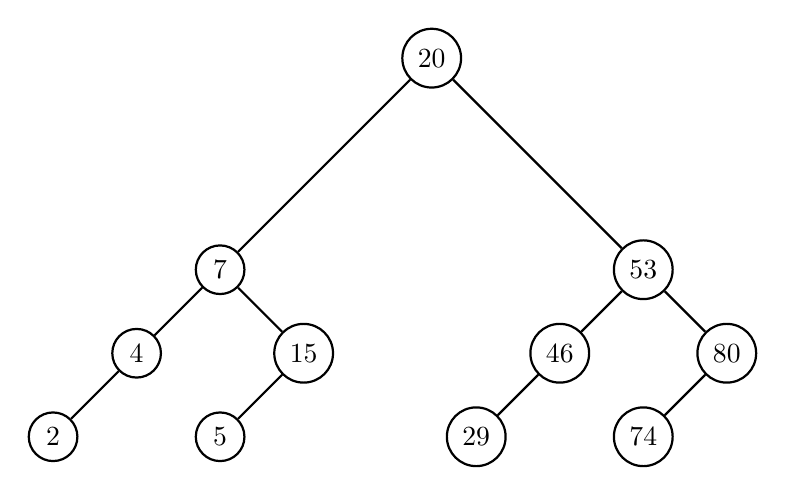
\begin{tikzpicture}[node distance={1.5cm}, thick, main/.style = {draw, circle}] 
    \node[main] (20) {20}; 
    \node[main] (7) [below left of = 20, node distance={3.8cm}] {7}; 
    \node[main] (53) [below right of = 20, node distance={3.8cm}] {53}; 
    \node[main] (4) [below left of = 7] {4}; 
    \node[main] (15) [below right of = 7] {15}; 
    \node[main] (2) [below left of = 4] {2}; 
    \node[main] (5) [below left of =  15] {5}; 
    \node[main] (46) [below left of = 53] {46}; 
    \node[main] (80) [below  right of = 53] {80}; 
    \node[main] (29) [below left of = 46] {29}; 
    \node[main] (74) [below right of=  46] {74}; 
    \draw (20) -- (7); 
    \draw (20) -- (53); 
    \draw (7) -- (4); 
    \draw (7) -- (15); 
    \draw (4) -- (2); 
    \draw (15) -- (5);
    \draw (53) -- (46);
    \draw (53) -- (80);
    \draw (46) -- (29);
    \draw (80) -- (74);
    \end{tikzpicture} 
\end{center}


    \end{center}
    \begin{lstlisting}[style=pythonstyle, language=Python]
def mystere(self):
    if self.gauche is None and self.droit is None:
        return 0
    elif self.gauche is None and self.droit is not None:
        return 1 + self.droit.mystere()
    elif self.gauche is not None and self.droit is None:
        return 1 + self.gauche.mystere()
    else:
        return 1 + max(self.droit.mystere(),self.gauche.mystere())
    \end{lstlisting}

    \Question Cet algorithme est-il récursif ?\\
\emptybox{1cm}
    \Question Donner un nouveau nom à la fonction mystère. Justifier. \\
    \emptybox{3cm}
    \Question En vous inspirant de l'exemple ci-dessus, écrivez une méthode taille retournant la taille de l'arbre. \\
    \emptybox{8cm}
    \Question Donner un code permettant de faire la somme des éléments dans le sous-arbre droit d'un nœud. (Indice "def somme(self)")\\
    \emptybox{8cm}
\end{Exercise}
\pagebreak